\documentclass[12pt]{article}

% Language setting
% Replace `english' with e.g. `pathspanish' to change the document language
\usepackage[english]{babel}

% Set page size and margins
% Replace `letterpaper' with`a4paper' for UK/EU standard size
\usepackage[a4paper,top=2cm,bottom=2cm,left=3cm,right=3cm,marginparwidth=1.75cm]{geometry}

% Useful packages
\usepackage{amsmath}
\usepackage{graphicx}
\usepackage{subfig}
\usepackage[colorlinks=true, allcolors=black]{hyperref}

\begin{document}

%title
\title{\underline{Project report - AutoPylot}}
\date{March 2022}


\author{%
    \\
    Alexandre Girold\\
    Mickael Bobovitch \\
    Maxime Ellerbach \\
    Maxime Gay \\ \\
    Group: Autonomobile 
    }

\maketitle

\centerline{
\includegraphics[height=8cm]{../../logos/logo-transparent-black.png}}
\newpage

\tableofcontents
\newpage

\section{Introduction}

\subsection{Project presentation}
Autonomous vehicles and more specifically self-driving cars have grasp the attention of many people for good or ill. In this spirit, we have decided with the Autonomobile team to create our first ever project, AutoPylot. The name of our team is of course full of meaning in that regard. Autonomobile is a two-word name, the first one a French word for autonomous : "Autonome", the second one a French word for car : "Automobile". These two-word combined literally mean Autonomous car.\\

What is AutoPylot's goal ? 
Drive itself on a track and win races. It may, at first glance seem very simple but not everything is at it seems. Yet we will try to make it as easy to understand as possible, without omitting crucial information. To achieve our goal, we need to solve many other problems. Those problems can be separate into two distinct groups. \\

The first one would be the software part. Indeed, in this project we will need to learn and acquire certain skills, from teamwork to coding in different languages. With those newly acquired skills we will be able to bring machine learning to our car to make it drive itself. This leads use directly to our second part, the more tangible one : hardware. Indeed, as we will progress in our work, we will need to see the results of our work in real life condition. This means implementing our code to a functioning car which will be able to race on a track. \\

This project will lead by a team of four young developers, Maxime Ellerbach, Mickael Bobovitch, Maxime Gay and Alexandre Girold. In this project work will be divided equally amongst all of us, sometimes we will have to work together to achieve our very tight time frame. 

\subsection{Team members}

% Write a small paragraph about yourself, what you like, what you did in the past. Everything is valuable !
\subsubsection{Maxime Ellerbach}
I am a curious and learning hungry person, always happy to learn and collaborate with new people ! Programming, robotics and tinkering has always attracted me. Writing code and then seeing the results in real life is something that I find amazing ! I had multiple projects in this field : Lego Mindstorms, a robotic arm, more recently an autonomous car and even a simulator in unity to train even without a circuit at home ! Even if I know quite well the domain of autonomous cars, there is always something new to learn. I look forward working with this team full of hard-working people on such a fun project !

\subsubsection{Mickael Bobovitch}
Roses are red. Violets are blue. Unexpected “Mickael BOBOVITCH“ on line 32. Hello I am a French Student with Russian parents. Lived half of my life in Moscow. Passionate in web dev, servers, and business. Started programming at 13 years old. Created many projects. I like to learn everything, from AI, to UI, from Hardware to Software. Actually I am like OCaml, you need to know me well to appreciate me.

\subsubsection{Maxime Gay}
I am 18 years old,  and I am crazy about investment, finance and especially cryptocurrencies and blockchain. I already worked with a team on different Investment projects and during summer Jobs, but this is the first time that I am working on such a  project. Furthermore, I am a beginner in computer Science and autonomous car. However, I am impatient to learn new skills with this incredible team. 

\subsubsection{Alexandre Girold}
I am already getting old. I am 19 years of age, yet I am full of resources. I am delighted to be able to learn something new. There are many things which I enjoy from programming to geopolitics. I know this project will push me toward a better me and make great friends along the way. 

\subsection{State of the art}
In this section, we will try to see what was previously made in this sector of industry.
It would not be realistic to compare our 1:10 project to real sized cars such as Tesla's, simply because in a racing environment,
we don't need to deal with such an amount of safety: pedestrian detection, emergency braking, speed limit detection and other.
So we will only see miniature autonomous racing framework that we would likely race against.\\

The most known is called "DonkeyCar", created by Will Roscoe and Adam Conway in early of 2017. Most of the models trained with DonkeyCar are behavior cloning models, meaning models that tries to replicate the behavior of a driver. This method uses a big amount of images (input) associated to steering angles and throttle (output), it requires the user to drive the car (collect data) prior to training the model: no examples means no training. The lack of training data often leads to the car leaving the track.\\

One other framework worth looking at is one created by Nvidia called "JetRacer" released in 2019. It uses a different approach from DonkeyCar where the user annotates the images by hand by clicking on where the car should go. The model used is similar to what DonkeyCar uses: a Convolutional Neural Network with one input (the image) and two outputs, one for the steering angle and one for the throttle to apply. \\

Both of those frameworks are written in python and use packages such as Tensorflow and OpenCV, we will also use them in our project.
\newpage



\section{Realized tasks}
% TODO

% Bobovitch
\subsection{Telemetry Server}

% Ellerbach
\subsection{Some theory}
Before going further into the DeepLearning part, let's have a quick reminder of what is a Neural Network and a bit of theory behind all of that. \\

\subsubsection{Neural Network}
So, what is a Neural Network ? 
A Neural Network or `NN` or `NeuralNet` for short is a black box. The role of a Neural Network is to approximate functions. This can be accomplished with a combination of layers that can be also seen as functions with N parameters and P outputs. Each layer can communicates with the next ones. In most architectures the Neural Network can be visualized as a sequential list of layers but some are more complex featuring: branches, feedforward and other mystical tricks. \\

This Neural Network by default is only outputing random results, to train it to best approximate our imaginary function, we need one thing: Data ! In our case, we need to predict the next action of our car: steering and throttle from an image: the POV of the car. We can also imagine adding other parameters to our black box like the current speed of the car.
During the training process, the prediction (Forward propagation) the model makes along with the expected value are used to correct the weights and inner parameters of every layers (Backward propagation). To have a well fitted Neural Network, the more the data we have and the best the quality of that data is, the better ! \\

NeuralNetworks are mainly composed of fully connected layers (or Dense layers), those are composed of a given amount of neurons. They receive one or more input signals, do calculation on them and then communicates its output signals to the next layer.\\

\centerline{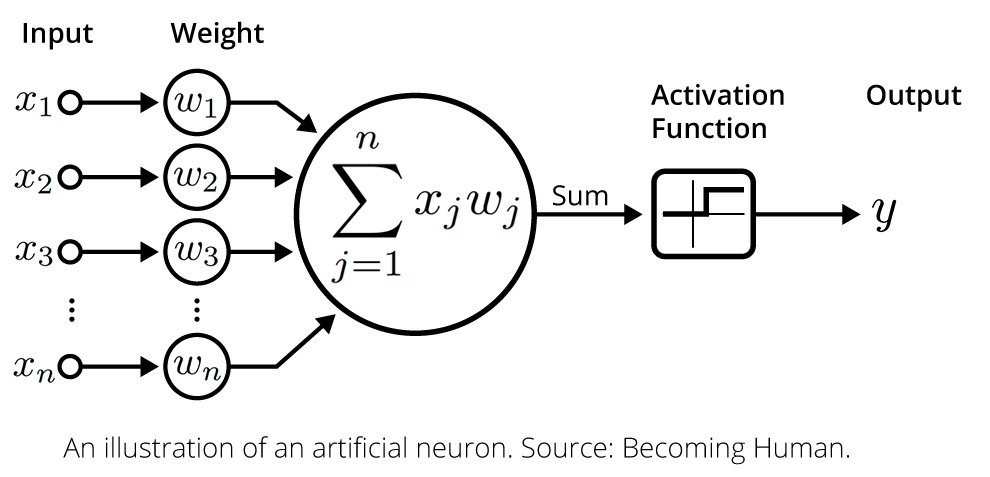
\includegraphics[height=8cm]{../../docs/activation-function.png}}

As you can see, the output signal is calculated from the sum of every input multiplied by its weight along with the addition of a bias. The output is then going through an activation function before outputing to the next layers. \\

\subsubsection{Convolutionnal Neural Network}
So now, what is a Convolutionnal Neural Network ?
First, a Convolutionnal Neural Network or `CNN` is a type of Neural Network ! It inherits it's name from the kind of layer it has: Convolution layers. \\

What is a Convolution ? 
A convolution is an operation that changes a function into something else. It uses kernels or filters to detect features in a signal. In our case, we use two dimensional convolution. The signal is the image composed of pixels (usually their values are between 255-0 or 1-0). The main idea behind having convolutions in a Neural Network is to analyze this signal and encode it into a smaller signal. \\
\centerline{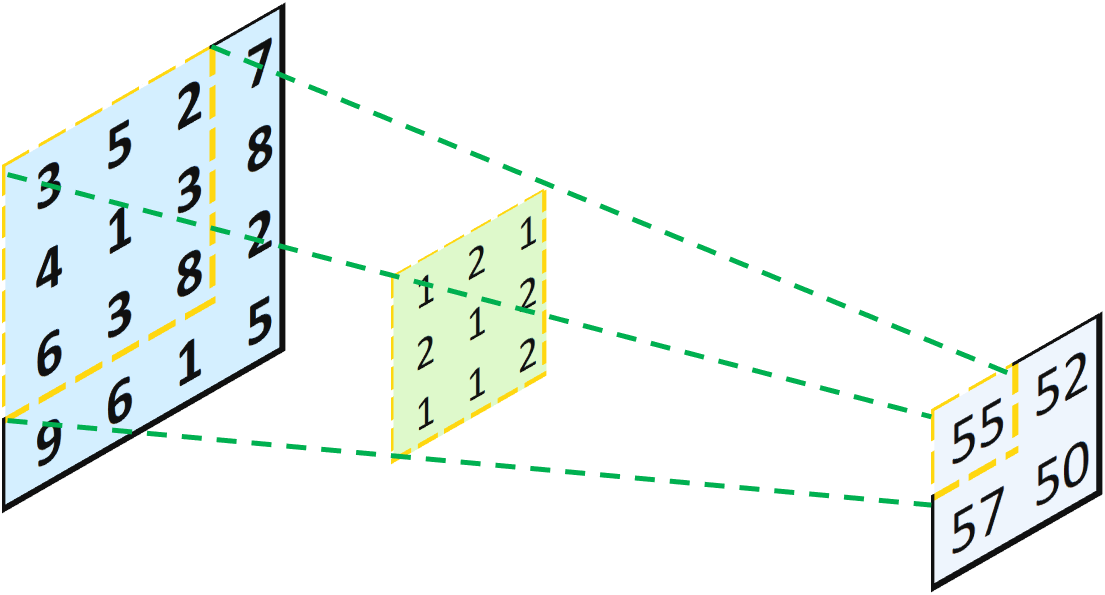
\includegraphics[height=8cm]{../../docs/convolution.png}}

Here you can see the application of a 3x3 convolution kernel on a 4x4 signal, the resulting of the application of this filter is a new signal of size 2x2. The resulting signal is smaller than the input signal, but why is that ? Simply because the kernel here is only applied on the valid areas of the input signal, so the outside border of the signal is lost. To prevent that, we can add zero values around the input filters so that the output size matches the input size. \\
\centerline{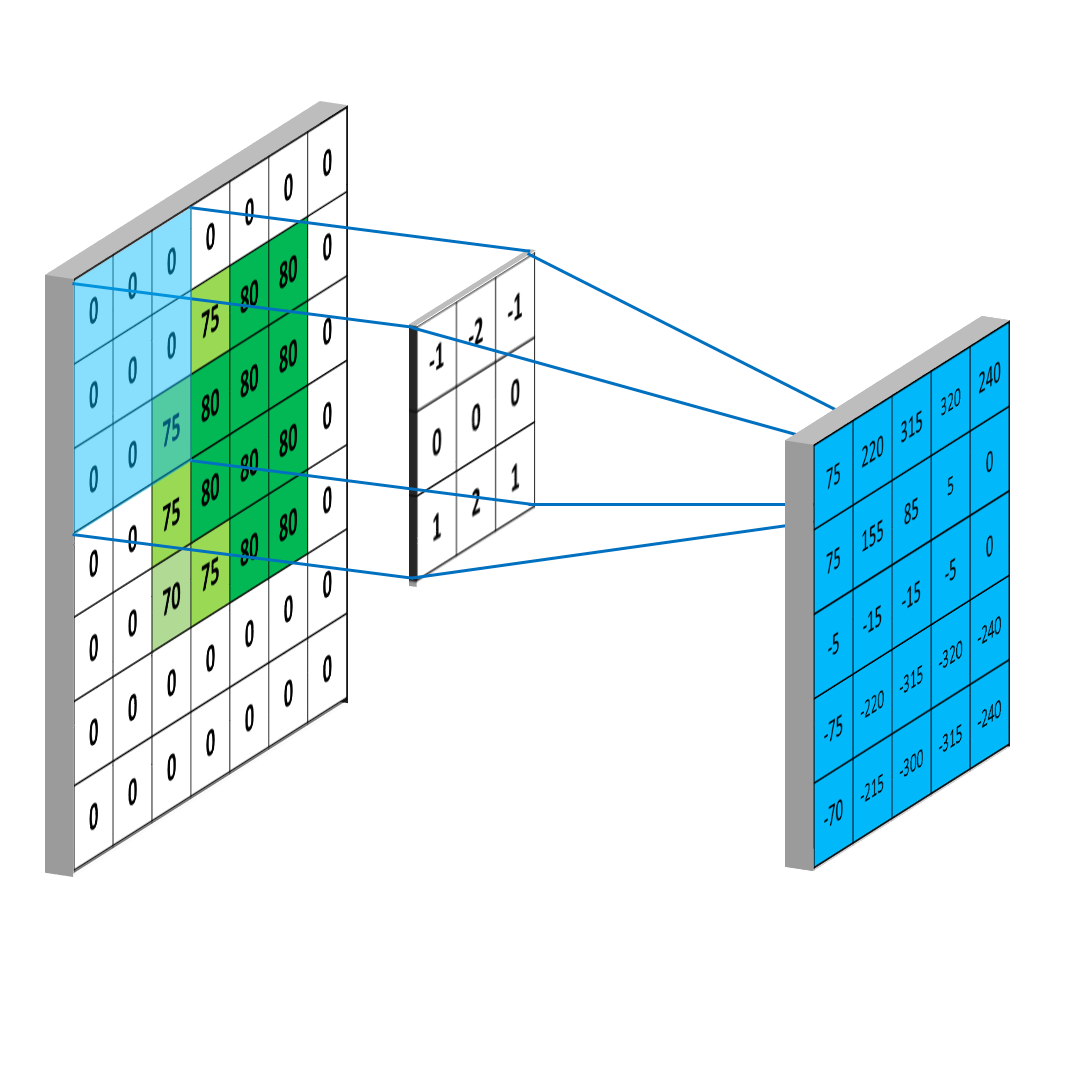
\includegraphics[height=8cm]{../../docs/padding.png}}

Now, as said previously, the main idea of having convolutions is to reduce the size of our image, this can be done by introducing strides to our convolution layers. The amount of movement between applications of the kernel of the input signal is reffered as the stride. On the above illustrations, we had a stride of 1 meaning at each step, the kernel moved by 1 pixel. On the illustration below, a 3x3 kernel is applied to a 5x5 signal with strides set to 2 without padding. This results in a 2x2 output signal. \\
\centerline{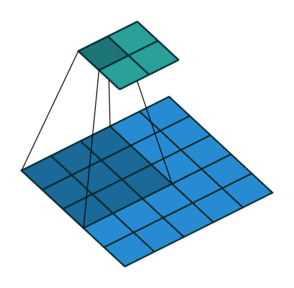
\includegraphics[height=6cm]{../../docs/strides.png}}

Each filter detects simple features from the previous signal but deepest the Convolutionnal Neural Network is, the more complex the detected features are. Here is an example where we are trying to detect the face of a dog in an image: 
The first convolution layer will detect simple features such as edges on the image, those can correspond to the shape of the dog as well as the shape of other stuff in the image. The second will have in input the already detected edges, from those edges it start could detect sets of edges looking like features coming from a dog: ears, eyes, fur. The third one will from those features detect even more complex features and so on.
After the convolutionnal layers, we are left with something called the latent space of our image. It is the encoded, simplified form of our image where only the key features are left. from those locally detected features, we can then have a look at the big picture by flattening the 2D signals into a 1D vector to be fed into fully connected layers and then answering the question ''Is there a dog in the image ?'' or ''Should we go right or left?''. \\


\subsubsection{Activation functions}
In some cases, we want our output signal to meet some requirements, for example, what if we only want outputs between -1 and 1 ? To answer this need, we apply some activation functions to the output of each layers. Here are some of the most popular activation functions. \\

Rectified Linear unit or `Relu` is the most widely used activation, it cuts off the negative values. It is defined as $ Relu(z) = \max(0, z)$. \\
\centerline{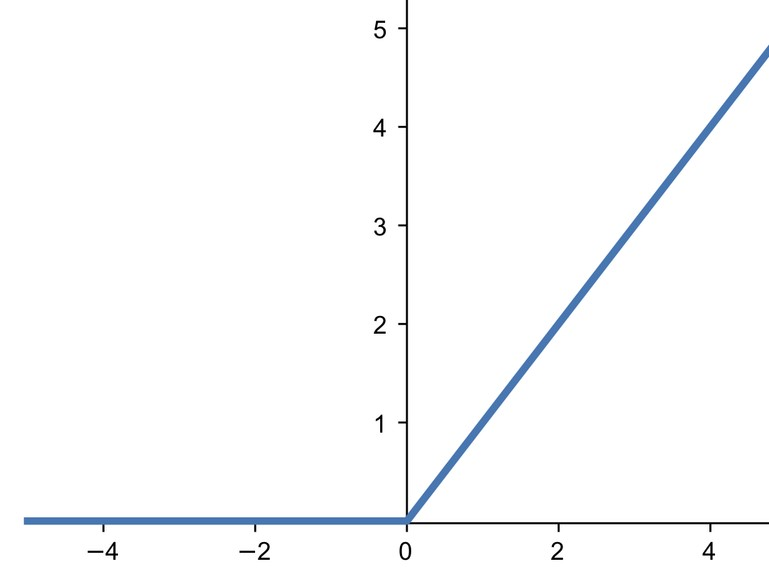
\includegraphics[height=6cm]{../../docs/relu.png}}

Sigmoid is an other widely used function, it maps every values between 0 and 1. It is defined as $ Sigmoid(z) = \frac{1} {1 + e^{-z}}$ \\
\centerline{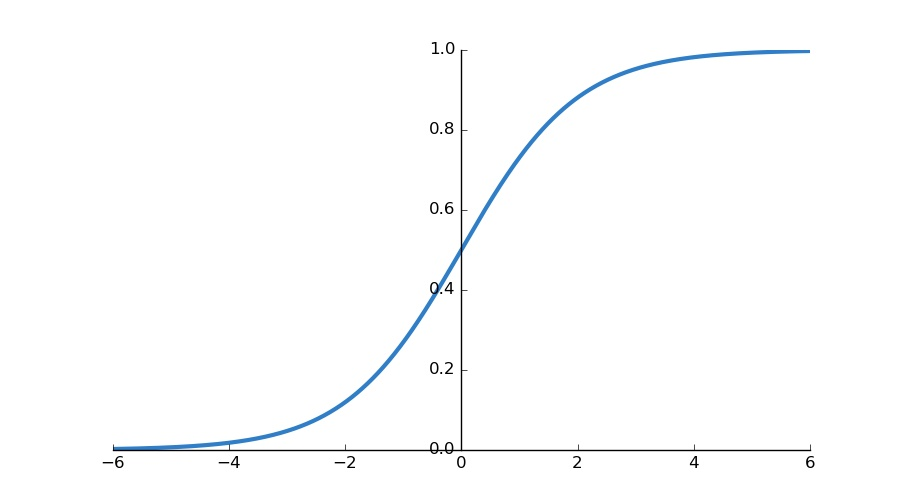
\includegraphics[height=6cm]{../../docs/sigmoid.png}}

Tanh, similarly to Sigmoid maps every values between -1 and 1. It is defined as $ Tanh(z) = \frac{1 - e^{-2z}}{1 + e^{-2z}}$ \\
\centerline{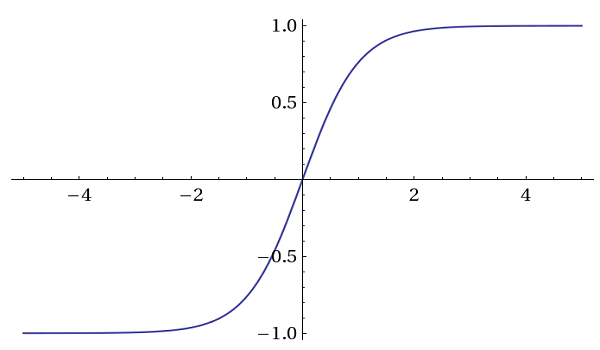
\includegraphics[height=6cm]{../../docs/tanh.png}}

\newpage

Softmax is mainly used for single label classification problems. It is defined as $ Softmax(z_i) = \frac{e^{z_{i}}}{\sum_{j=1}^K e^{z_{j}}} \ \ \ for\ i=1,2,\dots,K$ Note that the softmax activation can't be plotted as the activation of the current value depends on the other values.


% Everyone
\subsection{Model architectures}

So to summarize a bit what was said, a Convolutionnal Neural Network is a black box that have at least an image as an input and tries to predict something out of this image. As a common trend, the more convolution layers we have, the better our ouderstanding of the image will be. But we have to be carefull of how much we should put because we have to keep in mind the performance aspect of our model. In this section, you will see how every member of the team designed their model. \\

\subsubsection{Maxime Gay}
In order to create my model, I was inspired by the VGG-16 model.

This model was proposed by Karen Simonyan and Andrew Zisserman of the Visual Geometry Group Lab of Oxford University in 2014. It won the ImageNet Large Scale Visual Recognition Challenge (ILSVRC) the same year. The model achieves 92.7\% accuracy in ImageNet. By the way, ImageNet is a gigantic data base of more than 14 million of images. At this time, it was a sharp evolution regarding the other models because VGG-16 uses kernels of a smaller size.


Architecture of VGG-16 model :

\centerline{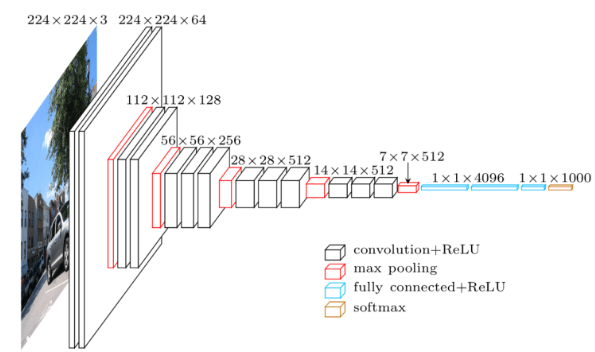
\includegraphics[height=8cm]{../../docs/VGG16.png}}


The VGG-16 architecture is composed of 13 convolutional layers with a 3x3 Kernel separated in five groups.

Between each group there is a pooling layer with a 2x2 size to reduce the size of the filter during the learning phase. At the end of those convolution and pooling layers, there are three Fully-Connected layers and an activation function softmax to determine the class of the image.


The problem of this model is that it is really slow and it is even slower in our case because it has to work with our car which does not have a lot of resources. Therefore, I decided to change the VGG-16 Model a little bit. 
I starte by removing some convolutional layers.

My first convolutional layer has a kernel of 5x5 and not 3x3 to have a filter with a bigger size at the beginning. Furthermore, I start with only four kernels on this first layer to reduce the cost of energy.

Then with the others layers, I increased progressively the number of kernels and I reduced the kernel size to 3x3. Moreover, I apply a stride of 2 for the first four layers and a stride of 1 for the last two. At the end, I use two Dense layers with an activation function "relu" like the others layers.


Furthermore, I tested many different optimizer like SGC, Adadelta, Nadam and Ftrl but I decided to use the Adam Optimizer because it gave me the best result. The Adam optimizer involves a combination of two gradient descent methodologies.

\centerline{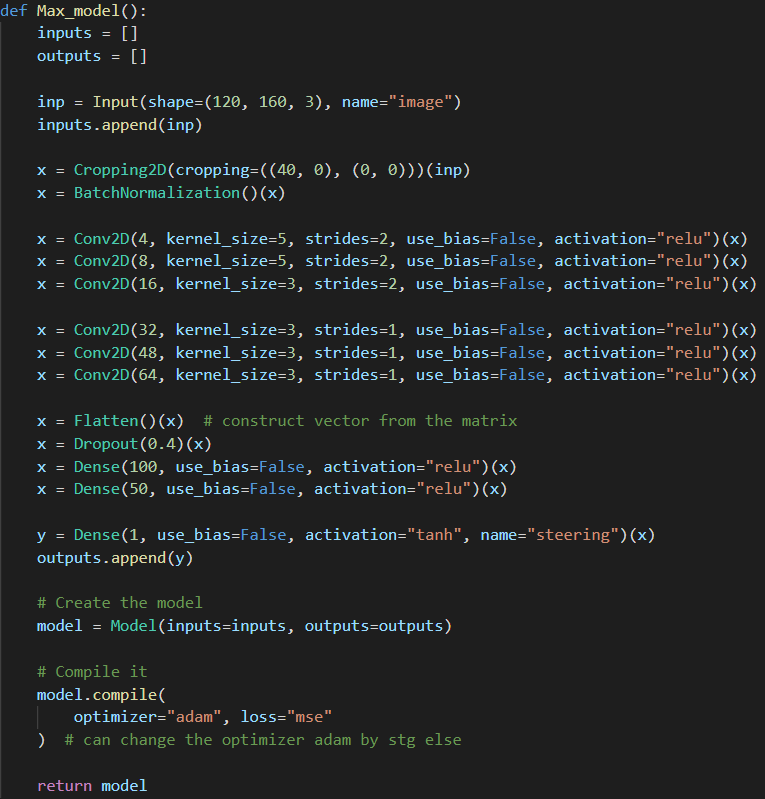
\includegraphics[height=8cm]{../../docs/model maxg.png}}


\subsubsection{Mickael Bobovitch}
\subsubsection{Alexandre Girold}
\subsubsection{Maxime Ellerbach}


% Ellerbach
\subsection{Model wrappers}

% Girold & Gay
\subsection{Load data during training}

% Girold
\subsection{Training Process}

After loading our data, we need to be able to train on those loaded data. The training process is where everything takes place. Indeed, training the data requires the use of all the previous functions. One of these functions is the settings.py. 

This function is the backbone of the training process. It allows us to have a very modular project where everything can be modified from this file only. This allow us to modify our project without deleting a lot of code, making it very modular which was one of our goals from the beginning. For example, we have recently added the telemetry server's restart function, once it was created, we only had to add it to the settings.py and all the other functions would be able to use it.   
This is also useful to change values in real-time. For example, if we want to train our model on more epochs or that our computer can handle bigger batch sizes then we only must change one value and that is it. This goes for all the functions in our project. 

\centerline{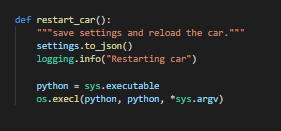
\includegraphics[height=8cm]{../../docs/restart-settings.png}}

The second import function is of course the train.py function.

At first, this function creates all our useful variables (imported from the settings).  Then if the given model doesn’t exist, we create it, for now, this model hasn’t yet been trained.  Then we need to feed the make sure all the variables are correct so the model can be trained.  To train a model we need data, in our case images. For this we need to make sure those data exist, and that the path to them is correct.  
We also want to know all the inputs and outputs. This is important as we might want to train not only the steering but also the throttle and speed.  
Finally, we use one important training library. The .fit library from karas. With fit, we are first feeding the training data(X) and training labels(Y) in our case these X and Y come from DataGenerator. We then use Keras to allow our model to train for a given number of epochs and on a given amount of batch sizes. 

% Bobovitch
\subsection{Data Augmentation}



\newpage

% sout : 7 / 03 & 25 / 04 & 06 / 06
\section {Planning}
\subsubsection {What is next ?}
The objectives we set ourselves for this presentation were acheived, for the next intermediate presentation we plan to finish what we are currently working on meaning The telemetry server and the logging. Moreover, we also plan to have a working prototype of the whole car including the AI part with the development of a basic convolutional neural network in a first time. This means we will have to create a model, then have a script to train it using collected data and finally a script to drive our car using this trained model.

\subsubsection {Races}

\begin{tabular}{|l|c|c|c|c|c|c|}
\hline
Tasks & Race 1 & Race 2 & Race 3 & Race 4 & Race 5 & Race 6  \\ 
\hline
Code controlled motors and servo                & 75\%   & 100\%  &        &        &        &         \\ 
\hline
Drive the car with a controller                 & 25\%   & 100\%   &        &        &        &         \\ 
\hline
Data collection                                 &        & 50\%   & 100\%  &        &        &         \\ 
\hline
Telemetry server                                &        & 25\%   & 100\%  &        &        &         \\ 
\hline
Logging                                         &        & 25\%   & 100\%  &        &        &         \\ 
\hline
Data processing and augmentation                &        &        & 50\%   & 75\%   & 100\%  &         \\ 
\hline
Basic Convolutional neural network              &        &        & 25\%   & 50\%   & 100\%  &         \\ 
\hline
\begin{tabular}[c]{@{}l@{}}Advanced \\models and optional objectives\end{tabular} &        &        &        &        &        & 50\%    \\
\hline
\end{tabular}

\subsection {Presentations}

\begin{tabular}{|l|c|c|c|} 
\hline
Tasks                                                                             & 1st presentation & 2nd Presentation & Final presentation  \\ 
\hline
Code controlled motors and servo                                                  & 100\%              &                &                    \\ 
\hline
Drive the car with a controller                                                   & 100\%              &                &                    \\ 
\hline
Data collection                                                                   & 75\%               & 100\%          &                    \\ 
\hline
Telemetry server                                                                  & 25\%               & 100\%          &                    \\ 
\hline
Logging                                                                           & 25\%               & 100\%          &                    \\ 
\hline
Presentation website                                                              & 100\%              & Update         & Update             \\ 
\hline
Data processing and augmentation                                                  &                    & 75\%           & 100\%              \\ 
\hline
Basic Convolutional neural network                                                &                    & 50\%           & 100\%              \\ 
\hline
\begin{tabular}[c]{@{}l@{}}Advanced \\models and optional objectives\end{tabular} &                    &                & 50\%               \\
\hline
\end{tabular}


\section {Task allocation}

\begin{tabular}{|l|c|c|c|c|} 
\hline
Tasks                        & Mickael B. & Maxime G. & Alexandre G. & Maxime E.  \\ 
\hline
Low level car control        &            &           &              & x          \\ 
\hline
Driving with a controller    &            & x         & x            & x          \\ 
\hline
Dataset handling             &            & x         & x            &            \\ 
\hline
Data processing              & x          & x         & x            & x          \\ 
\hline
Data visualization           &            &           &              & x          \\ 
\hline
Telemetry server             & x          &           &              & x          \\ 
\hline
Logging                      & x          &           &              & x          \\ 
\hline
Presentation website         & x          &           &              &            \\ 
\hline
Convolutional neural network & x          & x         & x            & x          \\ 
\hline
Main control loop            & x          &           &              &            \\
\hline
\end{tabular}

\section {Conclusion}
To sum up, Autonomobile team improved the control of the car with controller, furthermore the data processing is working flawlessly allowing us to load and save images and metadata. Moreover, our presentation website is ready, it includes the presentation of the team, some links to download our project and even a road map. Nevertheless, the hardest part is yet to come, indeed we have to work on the AI part of the car and on the telemetry website to have it working by the next project defense.\\
The telemetry website is important in order to visualize data to know what is happening inside the car at any moment. We will have to work and learn a lot on this topic which is fascinating.\\

To make a long story short, we spent a lot of time on this project, which comport many sections that are important for the realization of this project, and we will do every thing to succeed. 


\end{document}
